\documentclass[11pt,twoside,a4paper]{article}
% http://www-h.eng.cam.ac.uk/help/tpl/textprocessing/latex_maths+pix/node6.html symboles de math
% http://fr.wikibooks.org/wiki/Programmation_LaTeX Programmation latex (wikibook)
%=========================== En-Tete =================================
%--- Insertion de paquetages (optionnel) ---
\usepackage[french]{babel}   % pour dire que le texte est en fran{\'e}ais
\usepackage{a4}	             % pour la taille   
\usepackage[T1]{fontenc}     % pour les font postscript
\usepackage{epsfig}          % pour gerer les images
%\usepackage{psfig}
\usepackage{amsmath, amsthm} % tres bon mode mathematique
\usepackage{amsfonts,amssymb}% permet la definition des ensembles
\usepackage{float}           % pour le placement des figure
\usepackage{verbatim}

\usepackage{longtable} % pour les tableaux de plusieurs pages

\usepackage[table]{xcolor} % couleur de fond des cellules de tableaux

\usepackage{lscape} % changement orientation page

\usepackage{eso-pic} %% mettre une image de fond
% http://forums.fedora-fr.org/viewtopic.php?pid=337748

%\usepackage{frbib} % enlever pour obtenir references en anglais
% --- style de page (pour les en-tete) ---
% \pagestyle{headings}

% % % en-tete et pieds de page configurables : fancyhdr.sty
% http://www.trustonme.net/didactels/250.html
% http://ww3.ac-poitiers.fr/math/tex/pratique/entete/entete.htm
% http://www.ctan.org/tex-archive/macros/latex/contrib/fancyhdr/fancyhdr.pdf
\usepackage{fancyhdr}
\pagestyle{fancy}
\fancyhf{}
\fancyhead[LE,RO]{\begin{center} \textbf{Magazine Senso / Rezo} \end{center}}
\fancyfoot[LE]{\thepage \hfill
\textit{Magazine Senso / Rezo} \hfill 
\includegraphics[width=0.5cm]{img/logo_glider.eps} }
\fancyfoot[RO]{
\includegraphics[width=0.5cm]{img/logo_glider.eps} \hfill
\textit{Magazine Senso / Rezo} \hfill \thepage}
\renewcommand{\headrulewidth}{0pt}
\renewcommand{\footrulewidth}{0.5pt}
\addtolength{\headheight}{0.5pt}
\fancypagestyle{plain}{
	\fancyhead{}
	\fancyfoot{}
	\renewcommand{\headrulewidth}{0pt}
}

%--- Definitions de nouvelles commandes ---
\newcommand{\N}{\mathbb{N}} % les entiers naturels

\newcommand\BackgroundPic{
	\put(0,0){
	\parbox[b][\paperheight]{\paperwidth}{%
	\vfill
	\centering
	\includegraphics[width=\paperwidth,height=\paperheight,keepaspectratio]{img/page_sensorezo.eps}%
	\vfill
}}}


%--- Pour le titre ---
\def\maketitle{%
	\begin{center}
		\begin{tabular}[c]{c|c}
			\textsc{\textbf{Magazine SENSO / REZO}}~\\[\baselineskip]~\\[\baselineskip]
			\emph{\textbf{Num�ro 0 (Septembre 2009)}}~\\[\baselineskip]~\\[\baselineskip]
			\emph{\textbf{Journal underground de l'InterWeb}}~\\[\baselineskip]~\\[\baselineskip]
			\textsc{Auteur Inconnu}~\\[\baselineskip]~\\[\baselineskip]
			& 
			
\includegraphics[width=3cm]{img/logo_glider.eps}~\\[\baselineskip]
		\end{tabular}
		% \\ \hline
		 	% % if more than one logo
			% 
\includegraphics[width=5cm]{img/logo_glider.eps}
			% 
\includegraphics[width=5cm]{img/logo_wifi.eps}
		% \\ \hline
		% \end{tabular}
			~\\[\baselineskip]~\\[\baselineskip]
			\Huge{Senso / Rezo}~\\[\baselineskip]
			\Large{Underground et InterWeb}~\\[\baselineskip]
		
		~\\[\baselineskip]
		~\\[\baselineskip]
	\large{
		\textsc{\textbf{<<In Interweb we Trust>>}}
		~\\[\baselineskip]
		<<titre personne>> : \texttt{Anne ONYME}~\\[\baselineskip]
		<<titre personne>> : \texttt{Jocelyn CONNU}~\\[\baselineskip]
		~\\[\baselineskip]
		\textit{Steal This Magazine : Anarchy, Underground, InterWeb !}
	}

	\end{center}

}%



%--- Pour le glossaire --- a defaut de \makeglossary ou d'utilisation d'index latex

\definecolor{verylightgray}{rgb}{0.8,0.8,0.8}
\def\makeglossaire{%
	\begin{center}

	\begin{tabular}{|>{\columncolor{verylightgray}} p{0.2\textwidth}|p{0.8\textwidth}|}

		\hline

		\textbf{BLAST} & 

			\begin{tabular}{p{0.8\textwidth}}

			Basic Local Alignment Search Tool \\

			\textit{algorithmes et logiciels pour l'alignement de s{\'e}quences et la recherche de similarit{\'e}s locales}

			\end{tabular} \\

		\hline

		\textbf{BNDB} & Biochemical NetWork DataBase \textit{(entrep{\^o}t de donn{\'e}es)} \\

		\hline

	\end{tabular}

\end{center}

}%

%============================= Corps =================================
\begin{document}

\AddToShipoutPicture{\BackgroundPic}
% \AddToShipoutPicture*{\put(0,0){\includegraphics[width=\paperwidth]{img/page_sensorezo.eps}}}

%ecrire le titre...
\maketitle
\setcounter{page}{0}
\thispagestyle{empty}
\clearpage

\setcounter{page}{0}
\thispagestyle{empty}
% ecrire la table des mati{\'e}res...
\tableofcontents

% ecrire la table des figures et celle des tableaux

\setcounter{page}{0}
\thispagestyle{empty}

~\\ \rule{10cm}{1mm}~\\

\listoffigures

~\\ \rule{10cm}{1mm}~\\

\listoftables
\clearpage

%% le contenu

% \rule{10cm}{0.5mm}~\\

\section*{Introduction\markboth{Introduction}{Introduction}}

\addcontentsline{toc}{section}{Introduction}


[...]~\\

\rule{10cm}{0.5mm}~\\


\clearpage



\section{Section}



\subsection{Sous-section}



\subsubsection{sous sous sous section}

[...]~\\

\subsubsection{sous sous sous section}


\begin{table}[ht]

	\begin{center}

		\begin{tabular}{|p{0.1\textwidth}|p{0.8\textwidth}|}

		\hline

			
\includegraphics[width=1cm]{img/logo_glider.eps}

			& 

			\textbf{GLIDER} est le logo des hacker, symbole repris du jeu de la vie (cavalier). \\

		\hline

			
\includegraphics[width=1cm]{img/logo_wifi.eps}

			& 

			\textbf{WIFI} est une technologie de connection sans fil. \\

		\hline

		\end{tabular}

	\end{center}

	\caption{Un tableau r{\'e}f{\'e}renc{\'e}}

	\label{tab:TabReference01}

\end{table}~\\



\clearpage

\subsection{Encore une sous-section}


\begin{figure}[H]
	\centerline {
\epsfig {file=img/tux.eps,width=15cm}}
	\caption{Une belle image}
	\label{fig:FigReference01}
\end{figure}

\clearpage


\section*{Abbr{\'e}viations\markboth{Abbr{\'e}viations}{Abbr{\'e}viations}}

\addcontentsline{toc}{section}{Abbr{\'e}viations}

%% voir en haut : sous la definition du titre : glossaire

\makeglossaire



\clearpage

\section*{Bibliographie\markboth{Bibliographie}{Bibliographie}}

\addcontentsline{toc}{section}{Bibliographie}
\nocite{*}
%toutes references biblio : 6 lettres + 2 chiffres
\bibliography{modele_sensorezo_biblio}
\bibliographystyle{frplain} % plain or frplain
\end{document}